%%%%\setbeamerfont{itemize/enumerate body}{size*={9}{11}}
%%%%\setbeamerfont{itemize/enumerate subbody}{size*={8}{10}}
%%%%\setbeamerfont{itemize/enumerate subsubbody}{size*={7}{9}}

\frame{%
\frametitle{Summary}
\begin{itemize}
\item xxx
\end{itemize}

\vfill
\begin{block}{\footnotesize References}
\bmhe, chapter 1.\\
\bceabook
\end{block}

}

\frame{%
\frametitle{Summary}
\begin{itemize}
\item xxx
\end{itemize}

\vfill
\begin{block}{\footnotesize References}
\bmhe, chapter 1.\\
\bceabook
\end{block}

}

\frame{%
\frametitle{Summary}
\begin{itemize}
\item xxx
\end{itemize}

\vfill
\begin{block}{\footnotesize References}
\bmhe, chapter 1.\\
\bceabook
\end{block}

}


\frame{
\frametitle{4.\ Uncertainty analysis
\hspace{0pt plus 1 filll} \small $\left[p(\bm\theta\mid e,c)\right.$ vs $\left. g_i(\theta_i)\right]$}
\begin{overprint}
%%%\vspace{7pt}

%%%%%%%%%%%%%%%%%%%%%%%%%%%%%%%%%%%%%%%%%%%%%%%%%
\onslide<1|handout:0>
\fontsize{7}{8}\selectfont
\begin{tabular}{ccc}
\textbf{\blue Parameters} & \textbf{\blue Model structure} & \textbf{\blue Decision analysis} \\
\begin{minipage}[l]{2.5cm}
\begin{center}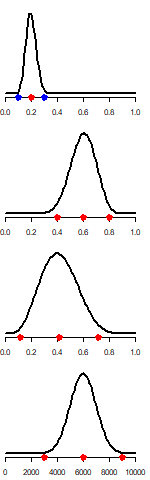
\includegraphics[scale=.37]{R/marginal-distns}\end{center}
\end{minipage}
&
\begin{minipage}[l]{5cm}
\begin{center}\red{Old chemotherapy}\black\end{center}\vspace{-.5cm}
\begin{center}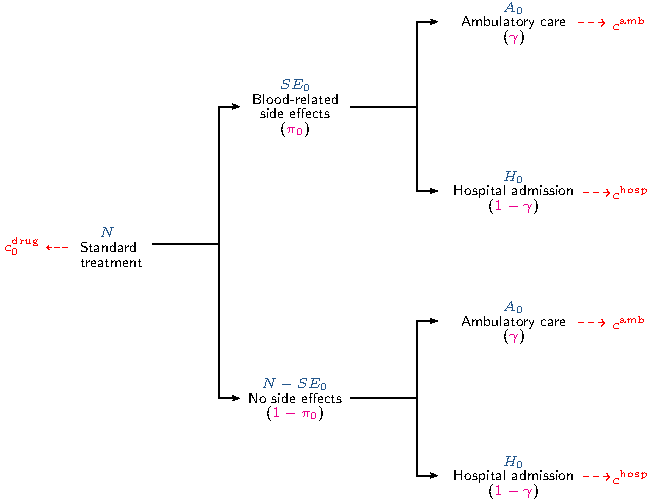
\includegraphics[scale=.37]{1.introduction-to-health-economic-evaluations/figs/ModelGraph2}\end{center}

\begin{center}\red{New chemotherapy}\black\end{center}\vspace{-.5cm}
\begin{center}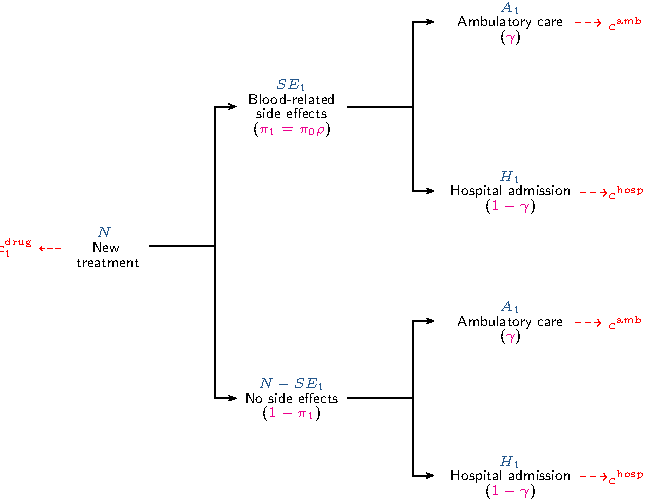
\includegraphics[scale=.37]{1.introduction-to-health-economic-evaluations/figs/ModelGraph4}\end{center}
\end{minipage}
&
\begin{minipage}[l]{4cm}
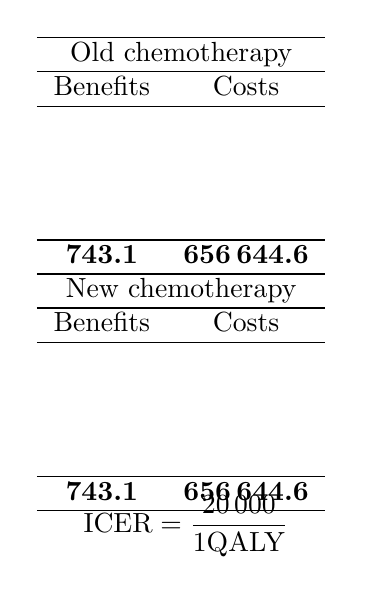
\begin{tikzpicture}
\draw(2.5,2) node[align=center,draw=none]{
\begin{tabular}{cc}
\hline
\multicolumn{2}{c}{Old chemotherapy} \\
\hline
Benefits & Costs \\
\hline 
 &  \\
 &  \\
 &  \\
 &  \\
\hline
\textbf{\white 743.1} & \textbf{\white 656\,644.6} \\
\hline
\end{tabular}
};

\draw(2.5,-1) node[align=center,draw=none]{
\begin{tabular}{cc}
\hline
\multicolumn{2}{c}{New chemotherapy} \\
\hline
Benefits & Costs \\
\hline 
 &  \\
 &  \\
 &  \\
 &  \\
\hline
\textbf{\white 743.1} & \textbf{\white 656\,644.6} \\
\hline
\end{tabular}
};

\draw(2.5,-2.7) node(3){\white $\displaystyle \mbox{ICER} = \frac{\mbox{20\,000}}{\mbox{1QALY}}$\black};
\end{tikzpicture}
\end{minipage}
\end{tabular}

%%%%%%%%%%%%%%%%%%%%%%%%%%%%%%%%%%%%%%%%%%%%%%%%%
\onslide<2|handout:0>
\fontsize{7}{8}\selectfont
\begin{tabular}{ccc}
\textbf{\blue Parameters} & \textbf{\blue Model structure} & \textbf{\blue Decision analysis} \\
\begin{minipage}[l]{2.5cm}
\begin{center}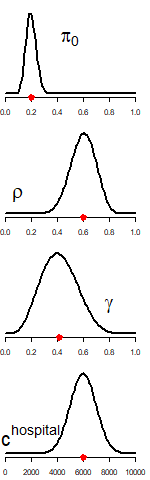
\includegraphics[scale=.37]{R/means-only}\end{center}
\end{minipage}
&
\begin{minipage}[l]{5cm}
\begin{center}\red{Old chemotherapy}\black\end{center}\vspace{-.5cm}
\begin{center}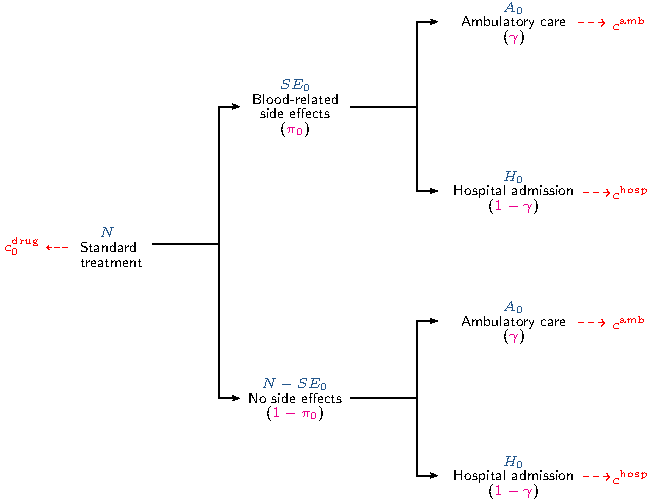
\includegraphics[scale=.37]{1.introduction-to-health-economic-evaluations/figs/ModelGraph2}\end{center}

\begin{center}\red{New chemotherapy}\black\end{center}\vspace{-.5cm}
\begin{center}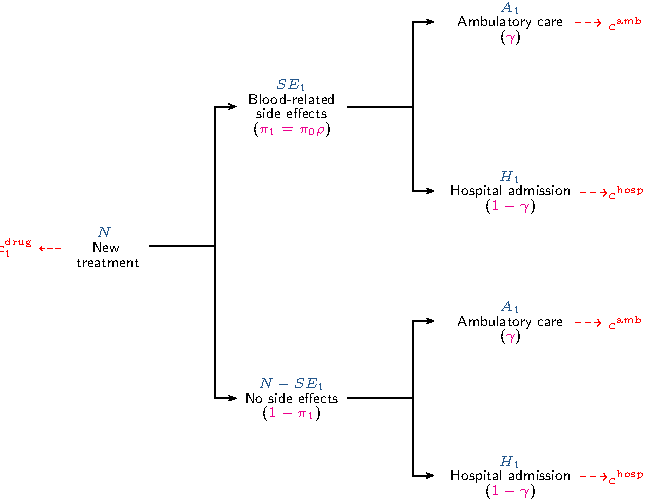
\includegraphics[scale=.37]{1.introduction-to-health-economic-evaluations/figs/ModelGraph4}\end{center}
\end{minipage}
&
\begin{minipage}[l]{4cm}
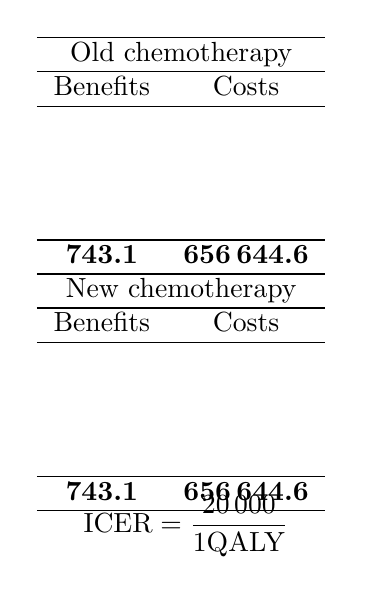
\begin{tikzpicture}
\draw(2.5,2) node[align=center,draw=none]{
\begin{tabular}{cc}
\hline
\multicolumn{2}{c}{Old chemotherapy} \\
\hline
Benefits & Costs \\
\hline 
 &  \\
 &  \\
 &  \\
 &  \\
\hline
\textbf{\white 743.1} & \textbf{\white 656\,644.6} \\
\hline
\end{tabular}
};

\draw(2.5,-1) node[align=center,draw=none]{
\begin{tabular}{cc}
\hline
\multicolumn{2}{c}{New chemotherapy} \\
\hline
Benefits & Costs \\
\hline 
 &  \\
 &  \\
 &  \\
 &  \\
\hline
\textbf{\white 743.1} & \textbf{\white 656\,644.6} \\
\hline
\end{tabular}
};

\draw(2.5,-2.7) node(3){\white $\displaystyle \mbox{ICER} = \frac{\mbox{20\,000}}{\mbox{1QALY}}$\black};
\end{tikzpicture}
\end{minipage}
\end{tabular}


%%%%%%%%%%%%%%%%%%%%%%%%%%%%%%%%%%%%%%%%%%%%%%%%%
\onslide<3|handout:0>
\fontsize{7}{8}\selectfont
\begin{tabular}{ccc}
\textbf{\blue Parameters} & \textbf{\blue Model structure} & \textbf{\blue Decision analysis} \\
\begin{minipage}[l]{2.5cm}
\begin{center}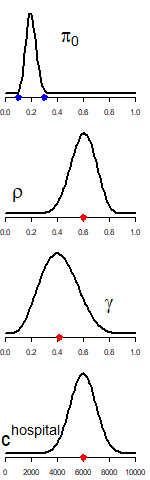
\includegraphics[scale=.37]{R/max-min-pi}\end{center}
\end{minipage}
&
\begin{minipage}[l]{5cm}
\begin{center}\red{Old chemotherapy}\black\end{center}\vspace{-.5cm}
\begin{center}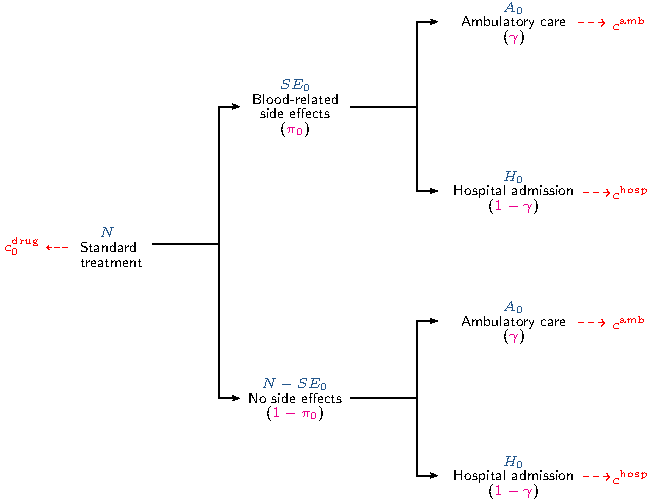
\includegraphics[scale=.37]{1.introduction-to-health-economic-evaluations/figs/ModelGraph2}\end{center}

\begin{center}\red{New chemotherapy}\black\end{center}\vspace{-.5cm}
\begin{center}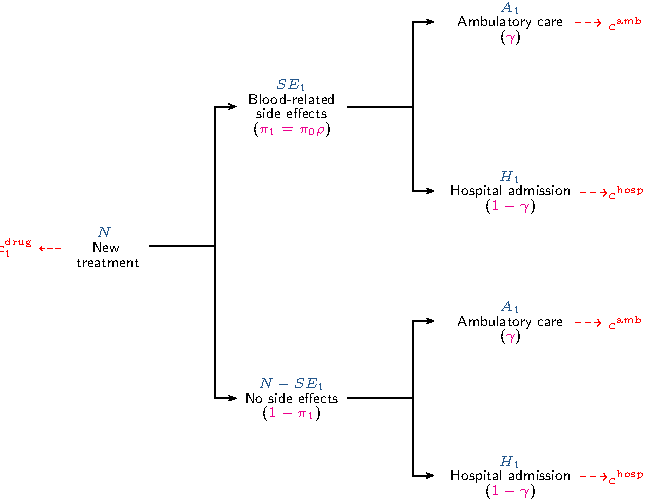
\includegraphics[scale=.37]{1.introduction-to-health-economic-evaluations/figs/ModelGraph4}\end{center}
\end{minipage}
&
\begin{minipage}[l]{4cm}
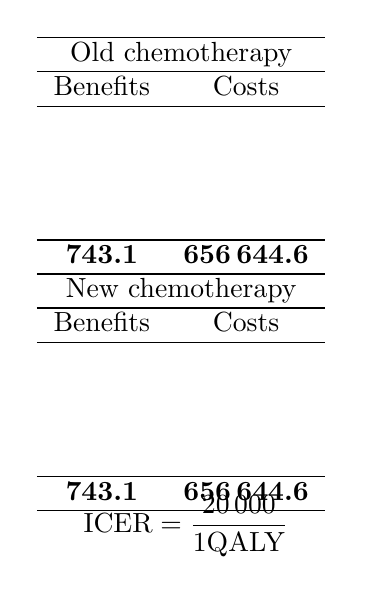
\begin{tikzpicture}
\draw(2.5,2) node[align=center,draw=none]{
\begin{tabular}{cc}
\hline
\multicolumn{2}{c}{Old chemotherapy} \\
\hline
Benefits & Costs \\
\hline 
 &  \\
 &  \\
 &  \\
 &  \\
\hline
\textbf{\white 743.1} & \textbf{\white 656\,644.6} \\
\hline
\end{tabular}
};

\draw(2.5,-1) node[align=center,draw=none]{
\begin{tabular}{cc}
\hline
\multicolumn{2}{c}{New chemotherapy} \\
\hline
Benefits & Costs \\
\hline 
 &  \\
 &  \\
 &  \\
 &  \\
\hline
\textbf{\white 743.1} & \textbf{\white 656\,644.6} \\
\hline
\end{tabular}
};

\draw(2.5,-2.7) node(3){\white $\displaystyle \mbox{ICER} = \frac{\mbox{20\,000}}{\mbox{1QALY}}$\black};
\end{tikzpicture}
\end{minipage}
\end{tabular}

%%%%%%%%%%%%%%%%%%%%%%%%%%%%%%%%%%%%%%%%%%%%%%%%%
\onslide<4|handout:0>
\fontsize{7}{8}\selectfont
\begin{tabular}{ccc}
\textbf{\blue Parameters} & \textbf{\blue Model structure} & \textbf{\blue Decision analysis} \\
\begin{minipage}[l]{2.5cm}
\begin{center}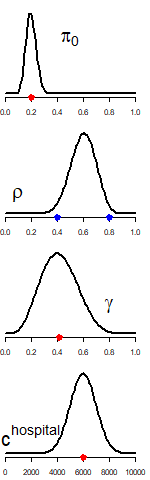
\includegraphics[scale=.37]{R/max-min-rho}\end{center}
\end{minipage}
&
\begin{minipage}[l]{5cm}
\begin{center}\red{Old chemotherapy}\black\end{center}\vspace{-.5cm}
\begin{center}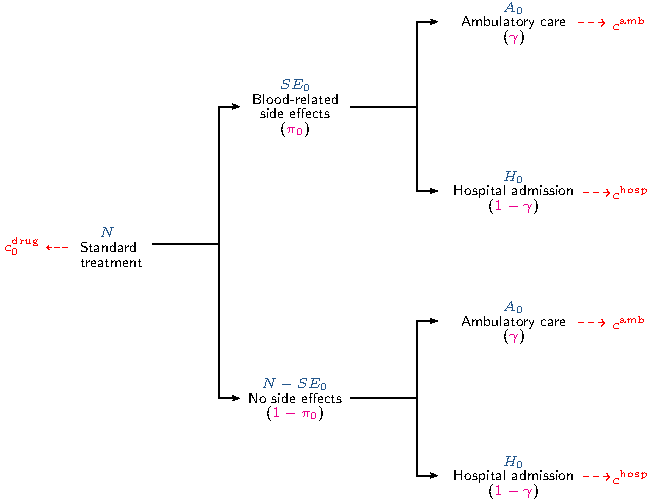
\includegraphics[scale=.37]{1.introduction-to-health-economic-evaluations/figs/ModelGraph2}\end{center}

\begin{center}\red{New chemotherapy}\black\end{center}\vspace{-.5cm}
\begin{center}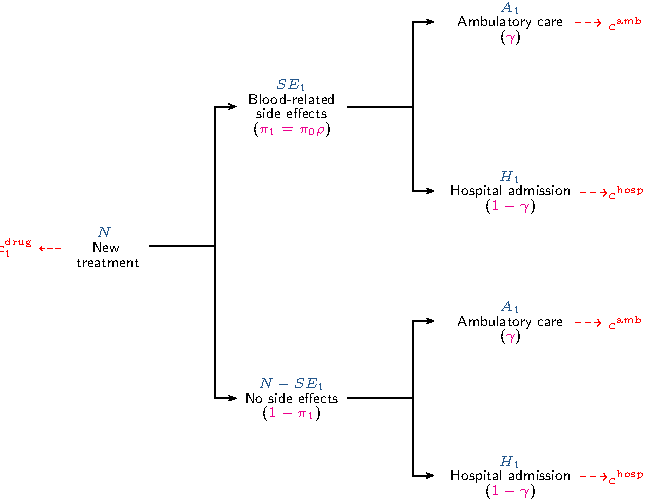
\includegraphics[scale=.37]{1.introduction-to-health-economic-evaluations/figs/ModelGraph4}\end{center}
\end{minipage}
&
\begin{minipage}[l]{4cm}
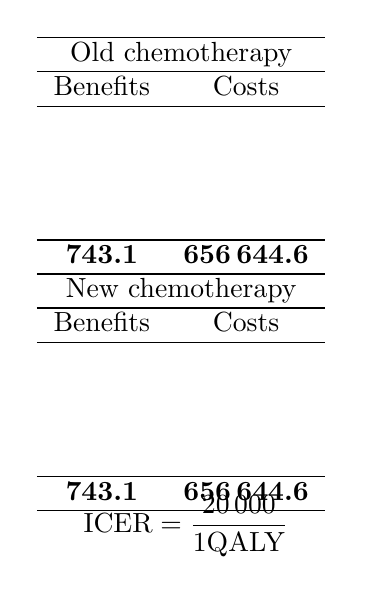
\begin{tikzpicture}
\draw(2.5,2) node[align=center,draw=none]{
\begin{tabular}{cc}
\hline
\multicolumn{2}{c}{Old chemotherapy} \\
\hline
Benefits & Costs \\
\hline 
 &  \\
 &  \\
 &  \\
 &  \\
\hline
\textbf{\white 743.1} & \textbf{\white 656\,644.6} \\
\hline
\end{tabular}
};

\draw(2.5,-1) node[align=center,draw=none]{
\begin{tabular}{cc}
\hline
\multicolumn{2}{c}{New chemotherapy} \\
\hline
Benefits & Costs \\
\hline 
 &  \\
 &  \\
 &  \\
 &  \\
\hline
\textbf{\white 743.1} & \textbf{\white 656\,644.6} \\
\hline
\end{tabular}
};

\draw(2.5,-2.7) node(3){\white $\displaystyle \mbox{ICER} = \frac{\mbox{20\,000}}{\mbox{1QALY}}$\black};
\end{tikzpicture}
\end{minipage}
\end{tabular}

%%%%%%%%%%%%%%%%%%%%%%%%%%%%%%%%%%%%%%%
\onslide<5|handout:0>
\fontsize{7}{8}\selectfont
\begin{tabular}{ccc}
\textbf{\blue Parameters} & \textbf{\blue Model structure} & \textbf{\blue Decision analysis} \\
\begin{minipage}[l]{2.5cm}
\begin{tikzpicture}
\draw(0,5) node{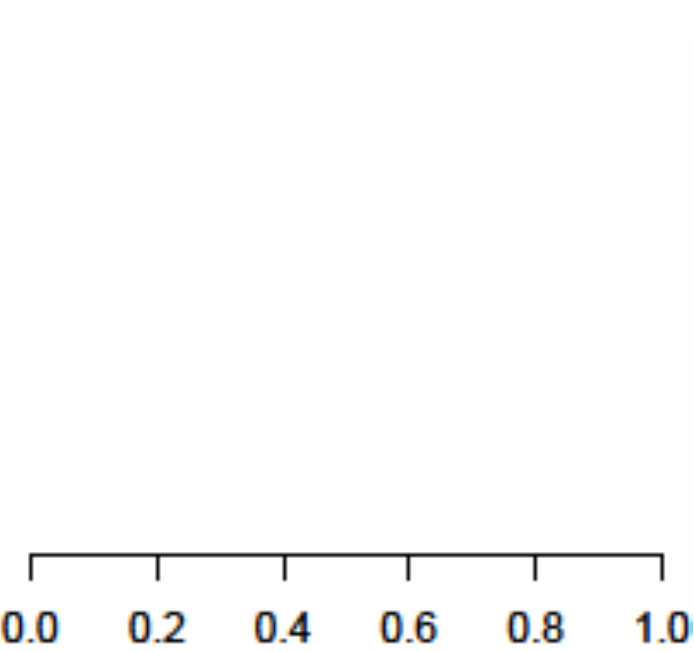
\includegraphics[scale=.35]{1.introduction-to-health-economic-evaluations/figs/pi0_grid}};
%\draw(0,5) node{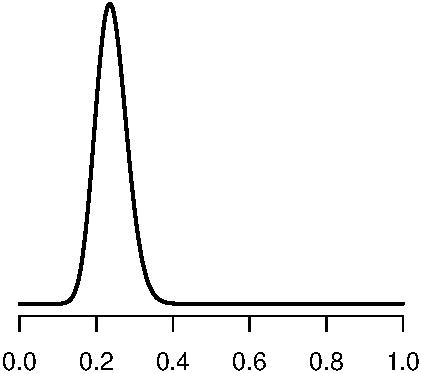
\includegraphics[scale=.27]{1.introduction-to-health-economic-evaluations/figs/pi0}};
\draw(0,3) node{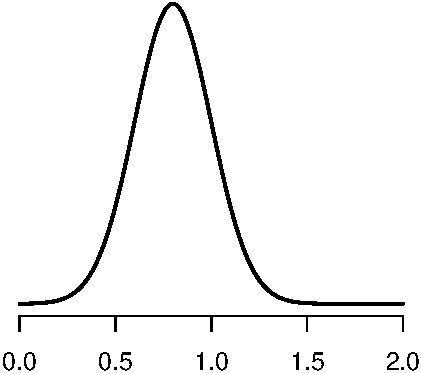
\includegraphics[scale=.27]{1.introduction-to-health-economic-evaluations/figs/rho}};
\draw(0,1) node{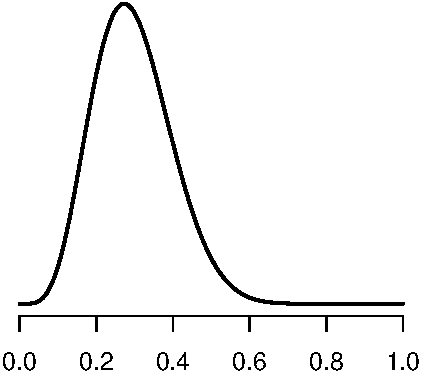
\includegraphics[scale=.27]{1.introduction-to-health-economic-evaluations/figs/gamma}};
\draw(0,-1) node{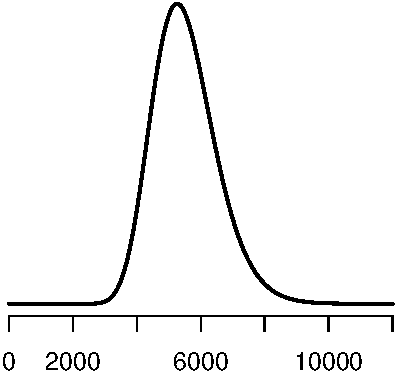
\includegraphics[scale=.27]{1.introduction-to-health-economic-evaluations/figs/chosp}};

\draw(0,5) node[align=center,draw=none,font=\fontsize{6}{7}\selectfont](1){$\pi_0$};
\draw(0.25,3) node[align=center,draw=none,font=\fontsize{6}{7}\selectfont](2){$\rho$};
\draw(.1,1.2) node[align=center,draw=none,font=\fontsize{6}{7}\selectfont](3){$\gamma$};
\draw(.5,-1.1) node[align=center,draw=none,font=\fontsize{6}{7}\selectfont](4){$c^{\rm{hosp}}$};


\draw(-0.7, 4.4) node[align=center,draw=none,color=black,font=\fontsize{7}{7}\selectfont]{\textbf{x}};
\draw(-0.4, 4.4) node[align=center,draw=none,color=black,font=\fontsize{7}{7}\selectfont]{\textbf{x}};
\draw(0, 4.4) node[align=center,draw=none,color=black,font=\fontsize{7}{7}\selectfont]{\textbf{x}};
\draw(0.6, 4.4) node[align=center,draw=none,color=black,font=\fontsize{7}{7}\selectfont]{\textbf{x}};

\draw(-0.6, 2.4) node[align=center,draw=none,color=gray,font=\fontsize{7}{7}\selectfont]{\textbf{x}};
\draw(-0.1, 2.4) node[align=center,draw=none,color=black,font=\fontsize{7}{7}\selectfont]{\textbf{x}};
\draw(0.3, 2.4) node[align=center,draw=none,color=gray,font=\fontsize{7}{7}\selectfont]{\textbf{x}};

\draw(0, 4.4) node[align=center,draw=none,color=red,font=\fontsize{7}{7}\selectfont]{\textbf{x}};
\draw(-.52,2.4) node[align=center,draw=none,color=red,font=\fontsize{7}{7}\selectfont]{\textbf{x}};
\draw(-.2,.4) node[align=center,draw=none,color=red,font=\fontsize{7}{7}\selectfont]{\textbf{x}};
\draw(-.6,-1.6) node[align=center,draw=none,color=red,font=\fontsize{7}{7}\selectfont]{\textbf{x}};
\end{tikzpicture}
\end{minipage}
&
\begin{minipage}[l]{5cm}
\begin{center}\red{Old chemotherapy}\black\end{center}\vspace{-.5cm}
\begin{center}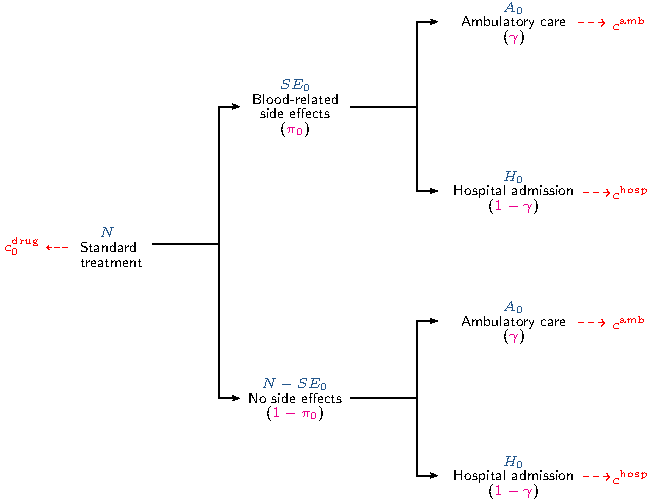
\includegraphics[scale=.37]{1.introduction-to-health-economic-evaluations/figs/ModelGraph2}\end{center}

\begin{center}\red{New chemotherapy}\black\end{center}\vspace{-.5cm}
\begin{center}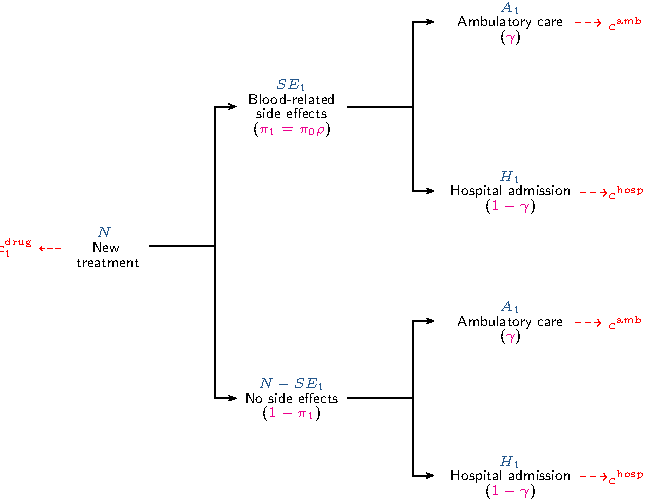
\includegraphics[scale=.37]{1.introduction-to-health-economic-evaluations/figs/ModelGraph4}\end{center}
\end{minipage}
&
\begin{minipage}[l]{4cm}
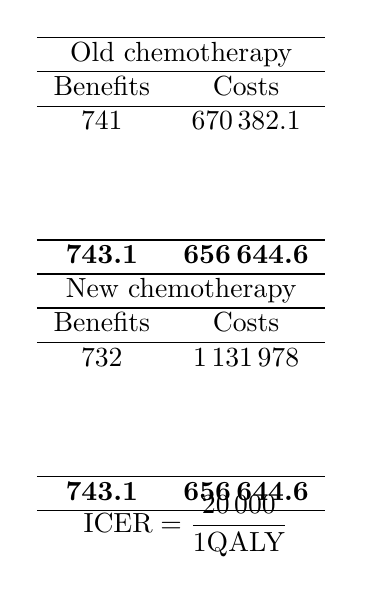
\begin{tikzpicture}
\draw(2.5,2) node[align=center,draw=none]{
\begin{tabular}{cc}
\hline
\multicolumn{2}{c}{Old chemotherapy} \\
\hline
Benefits & Costs \\
\hline 
741 & 670\,382.1 \\
 &  \\
 &  \\
 &  \\
\hline
\textbf{\white 743.1} & \textbf{\white 656\,644.6} \\
\hline
\end{tabular}
};

\draw(2.5,-1) node[align=center,draw=none]{
\begin{tabular}{cc}
\hline
\multicolumn{2}{c}{New chemotherapy} \\
\hline
Benefits & Costs \\
\hline 
732 & 1\,131\,978 \\
 &  \\
 &  \\
 &  \\
\hline
\textbf{\white 743.1} & \textbf{\white 656\,644.6} \\
\hline
\end{tabular}
};

\draw(2.5,-2.7) node(3){\white $\displaystyle \mbox{ICER} = \frac{\mbox{20\,000}}{\mbox{1QALY}}$\black};
%\draw(-5.5,.3) node(4){$\Rightarrow$};
%\draw(-0,.3) node(5){$\Rightarrow$};
\end{tikzpicture}
\end{minipage}
\end{tabular}


%%%%%%%%%%%%%%%%%%%%%%%%%%%%%%%%%%%%%%%
\onslide<6|handout:0>
\fontsize{7}{8}\selectfont
\begin{tabular}{ccc}
\textbf{\blue Parameters} & \textbf{\blue Model structure} & \textbf{\blue Decision analysis} \\
\begin{minipage}[l]{2.5cm}
\begin{tikzpicture}
\draw(0,5) node{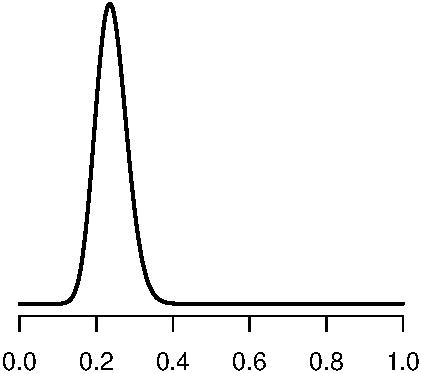
\includegraphics[scale=.27]{1.introduction-to-health-economic-evaluations/figs/pi0}};
\draw(0,3) node{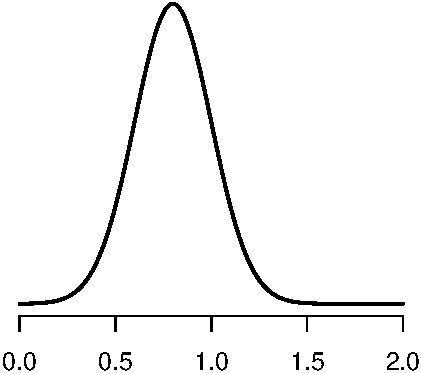
\includegraphics[scale=.27]{1.introduction-to-health-economic-evaluations/figs/rho}};
\draw(0,1) node{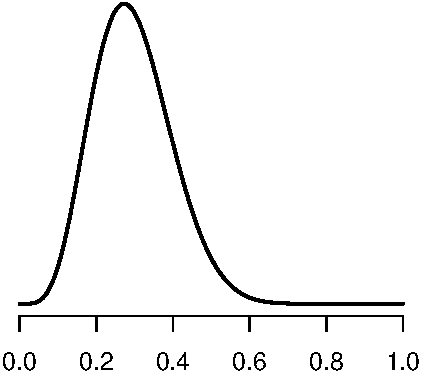
\includegraphics[scale=.27]{1.introduction-to-health-economic-evaluations/figs/gamma}};
\draw(0,-1) node{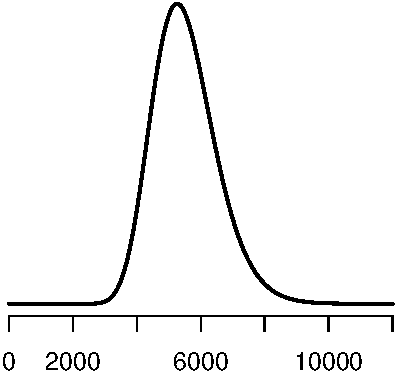
\includegraphics[scale=.27]{1.introduction-to-health-economic-evaluations/figs/chosp}};
\draw(0,5) node[align=center,draw=none,font=\fontsize{6}{7}\selectfont](1){$\pi_0$};
\draw(0.25,3) node[align=center,draw=none,font=\fontsize{6}{7}\selectfont](2){$\rho$};
\draw(.1,1.2) node[align=center,draw=none,font=\fontsize{6}{7}\selectfont](3){$\gamma$};
\draw(.5,-1.1) node[align=center,draw=none,font=\fontsize{6}{7}\selectfont](4){$c^{\rm{hosp}}$};
\draw(.15,4.4) node[align=center,draw=none,color=red,font=\fontsize{7}{7}\selectfont]{\textbf{x}};
\draw(-.32,2.4) node[align=center,draw=none,color=red,font=\fontsize{7}{7}\selectfont]{\textbf{x}};
\draw(.2,.4) node[align=center,draw=none,color=red,font=\fontsize{7}{7}\selectfont]{\textbf{x}};
\draw(-.1,-1.6) node[align=center,draw=none,color=red,font=\fontsize{7}{7}\selectfont]{\textbf{x}};
\end{tikzpicture}
\end{minipage}
&
\begin{minipage}[l]{5cm}
\begin{center}\red{Old chemotherapy}\black\end{center}\vspace{-.5cm}
\begin{center}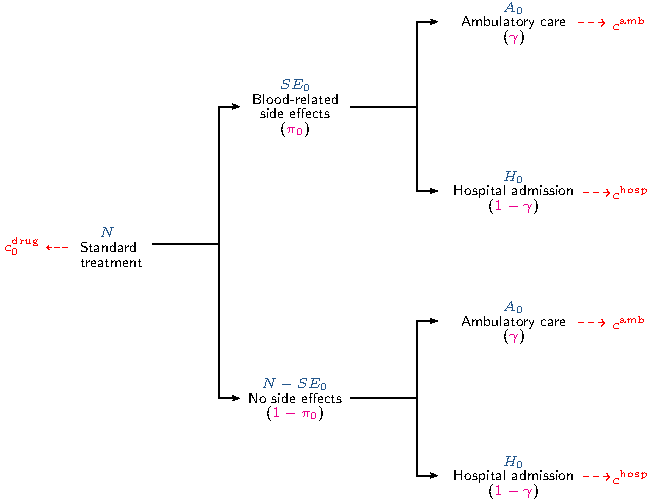
\includegraphics[scale=.37]{1.introduction-to-health-economic-evaluations/figs/ModelGraph2}\end{center}

\begin{center}\red{New chemotherapy}\black\end{center}\vspace{-.5cm}
\begin{center}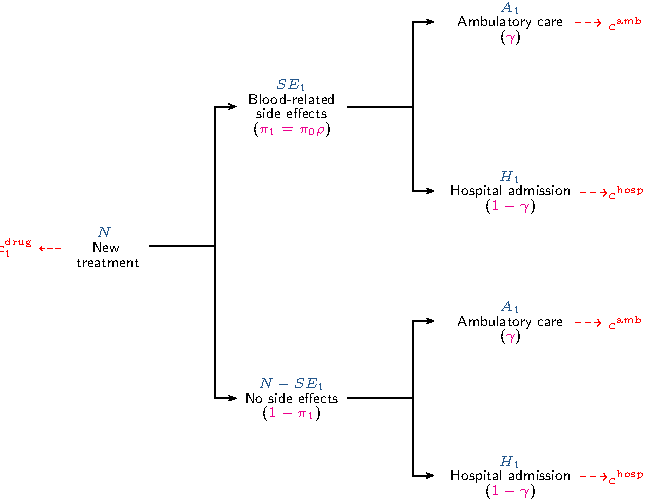
\includegraphics[scale=.37]{1.introduction-to-health-economic-evaluations/figs/ModelGraph4}\end{center}
\end{minipage}
&
\begin{minipage}[l]{4cm}
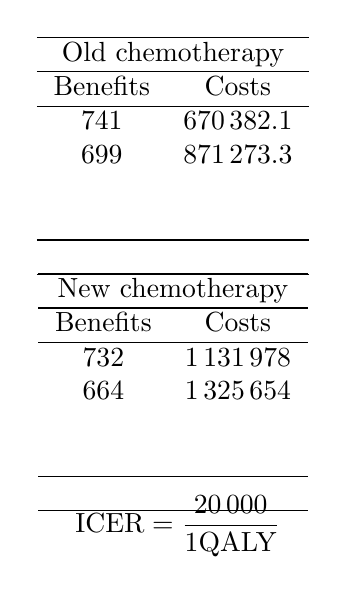
\begin{tikzpicture}
\draw(2.5,2) node[align=center,draw=none]{
\begin{tabular}{cc}
\hline
\multicolumn{2}{c}{Old chemotherapy} \\
\hline
Benefits & Costs \\
\hline 
741 & 670\,382.1 \\
699 & 871\,273.3 \\
 &  \\
 &  \\
\hline
 &  \\
\hline
\end{tabular}
};

\draw(2.5,-1) node[align=center,draw=none]{
\begin{tabular}{cc}
\hline
\multicolumn{2}{c}{New chemotherapy} \\
\hline
Benefits & Costs \\
\hline 
732 & 1\,131\,978 \\
664 & 1\,325\,654 \\
 &  \\
 &  \\
\hline
 &  \\
\hline
\end{tabular}
};

\draw(2.5,-2.7) node(3){\white $\displaystyle \mbox{ICER} = \frac{\mbox{20\,000}}{\mbox{1QALY}}$\black};
%\rput(-5.5,.3){$\Rightarrow$}
%\rput(-0,.3){$\Rightarrow$}
\end{tikzpicture}
\end{minipage}
\end{tabular}

\onslide<7|handout:1>
\fontsize{7}{8}\selectfont
\begin{tabular}{ccc}
\textbf{\blue Parameters} & \textbf{\blue Model structure} & \textbf{\blue Decision analysis} \\
\begin{minipage}[l]{2.5cm}
\begin{tikzpicture}
\draw(0,5) node{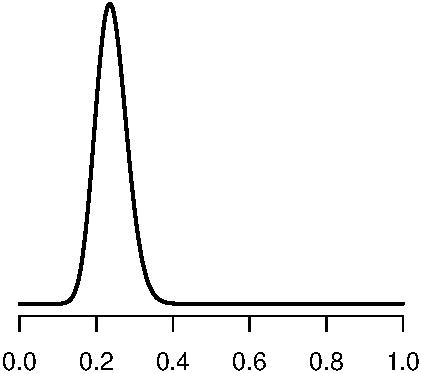
\includegraphics[scale=.27]{1.introduction-to-health-economic-evaluations/figs/pi0}};
\draw(0,3) node{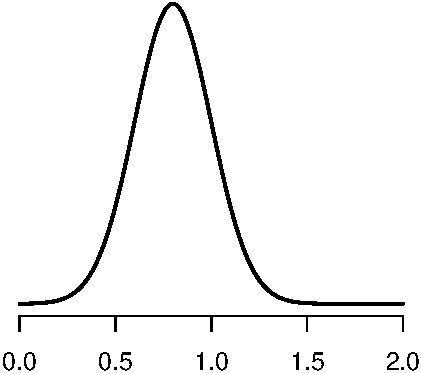
\includegraphics[scale=.27]{1.introduction-to-health-economic-evaluations/figs/rho}};
\draw(0,1) node{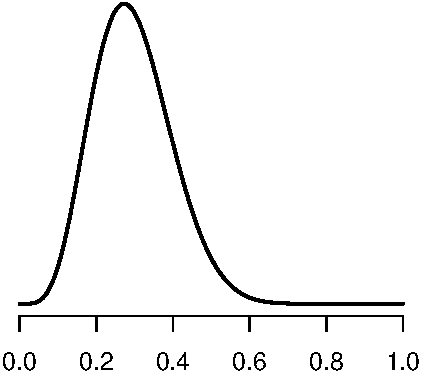
\includegraphics[scale=.27]{1.introduction-to-health-economic-evaluations/figs/gamma}};
\draw(0,-1) node{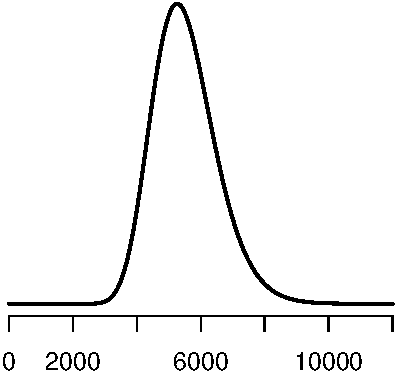
\includegraphics[scale=.27]{1.introduction-to-health-economic-evaluations/figs/chosp}};
\draw(0,5) node[align=center,draw=none,font=\fontsize{6}{7}\selectfont](1){$\pi_0$};
\draw(0.25,3) node[align=center,draw=none,font=\fontsize{6}{7}\selectfont](2){$\rho$};
\draw(.1,1.2) node[align=center,draw=none,font=\fontsize{6}{7}\selectfont](3){$\gamma$};
\draw(.5,-1.1) node[align=center,draw=none,font=\fontsize{6}{7}\selectfont](4){$c^{\rm{hosp}}$};
\draw(.25,4.4) node[align=center,draw=none,color=red,font=\fontsize{7}{7}\selectfont]{\textbf{x}};
\draw(.12,2.4) node[align=center,draw=none,color=red,font=\fontsize{7}{7}\selectfont]{\textbf{x}};
\draw(-.0,.4) node[align=center,draw=none,color=red,font=\fontsize{7}{7}\selectfont]{\textbf{x}};
\draw(.04,-1.6) node[align=center,draw=none,color=red,font=\fontsize{7}{7}\selectfont]{\textbf{x}};
\end{tikzpicture}
\end{minipage}
&
\begin{minipage}[l]{5cm}
\begin{center}\red{Old chemotherapy}\black\end{center}\vspace{-.5cm}
\begin{center}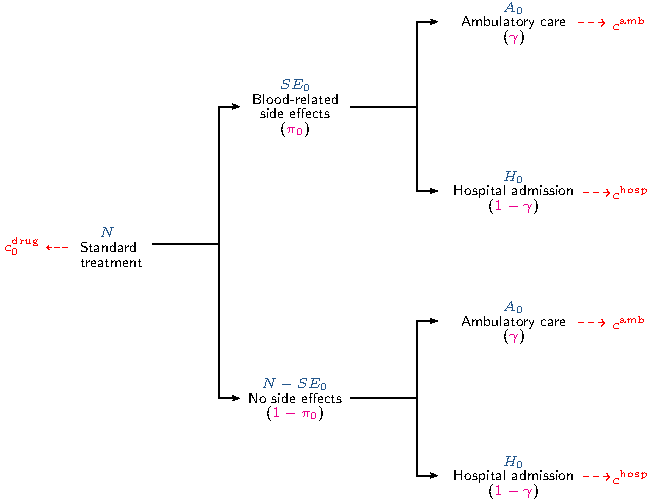
\includegraphics[scale=.37]{1.introduction-to-health-economic-evaluations/figs/ModelGraph2}\end{center}

\begin{center}\red{New chemotherapy}\black\end{center}\vspace{-.5cm}
\begin{center}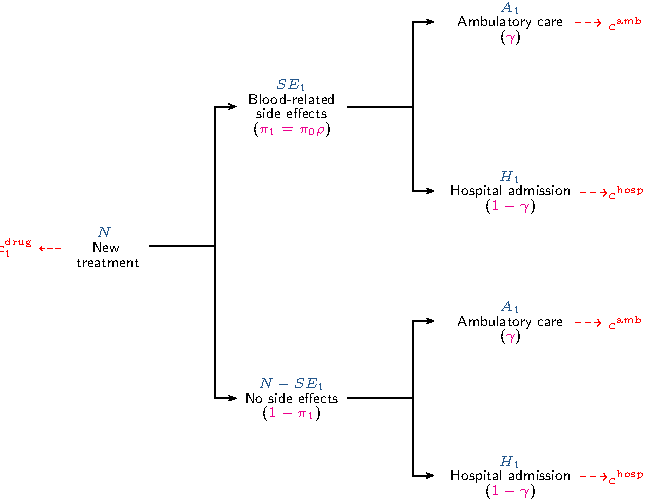
\includegraphics[scale=.37]{1.introduction-to-health-economic-evaluations/figs/ModelGraph4}\end{center}
\end{minipage}
&
\begin{minipage}[l]{4cm}
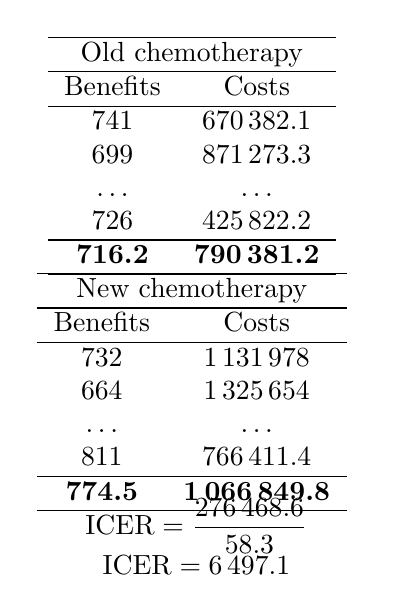
\begin{tikzpicture}
\draw(2.5,2) node[align=center,draw=none]{
\begin{tabular}{cc}
\hline
\multicolumn{2}{c}{Old chemotherapy} \\
\hline
Benefits & Costs \\
\hline 
741 & 670\,382.1 \\
699 & 871\,273.3 \\
$\ldots$ & $\ldots$ \\
726 & 425\,822.2 \\
\hline
\textbf{716.2} & \textbf{790\,381.2} \\
\hline
\end{tabular}
};

\draw(2.5,-1) node[align=center,draw=none]{
\begin{tabular}{cc}
\hline
\multicolumn{2}{c}{New chemotherapy} \\
\hline
Benefits & Costs \\
\hline 
732 & 1\,131\,978 \\
664 & 1\,325\,654 \\
$\ldots$ & $\ldots$ \\
811 & 766\,411.4 \\
\hline
\textbf{774.5} & \textbf{1\,066\,849.8} \\
\hline
\end{tabular}
};

\draw(2.5,-2.7) node(3){$\displaystyle \mbox{ICER} = \frac{\mbox{276\,468.6}}{\mbox{58.3}}$};
\draw(2.5,-3.2) node(3){$\displaystyle \mbox{\white ICER\black} = \mbox{6\,497.1}$};
%%%%
%%%%\rput(2,-2.7){$\displaystyle \mbox{ICER =} \frac{\mbox{276\,468.6}}{\mbox{58.3}}$}
%%%%\rput(2,-3.2){$\displaystyle \mbox{\white ICER\black =} \mbox{ 6\,497.1}$}
%%%%\rput(-5.5,.3){$\Rightarrow$}
%%%%\rput(-0,.3){$\Rightarrow$}
\end{tikzpicture}
\end{minipage}
\end{tabular}

\end{overprint}
}

\frame{
\frametitle{Is this \textit{all} we need? \hspace{0pt plus 1 filll}\small \textit{(see VoI)}}
\only<1-3|handout:1>{
\begin{itemize}
\item The CEAC only deals with the \textbf{\blue probability} of making the ``right decision''
\item But it does not account for the \textbf{\red payoff/penalty} associated with making the ``wrong''~one!
\vspace{10pt}
\item<2-3|handout:1> \textbf{Example 1}: Intervention $t=1$ is the most cost-effective, given current evidence
\begin{itemize}
\item<2-3|handout:1> \myblue $\Pr(\mbox{$t=1$ is cost-effective)}=$ 0.51 \black 
\item<2-3|handout:1> If we get it wrong: Increase in costs = \pounds 3
\item[]<2-3|handout:1> \white If we get it wrong: \black Decrease in effectiveness = 0.000001 QALYs
\item \red Large uncertainty\black/\color{blue!20!black!30!green} negligible consequences \black $\Rightarrow$ \textbf{\color{blue!20!black!30!green}can afford uncertainty}
\end{itemize}
\vspace{5pt}
\item<3|handout:1> \textbf{Example 2}: Intervention $t=1$ is the most cost-effective, given current evidence
\begin{itemize}
\item<3|handout:1> \myblue $\Pr(\mbox{$t=1$ is cost-effective)}=$ 0.999 \black 
\item<3|handout:1> If we get it wrong: Increase in costs = \pounds 1\,000\,000\,000
\item[]<3|handout:1> \white If we get it wrong: \black Decrease in effectiveness = 999999 QALYs
\item<3|handout:1> \color{blue!20!black!30!green} Tiny uncertainty\black/\red dire consequences \black $\Rightarrow$ \amber \textbf{probably should think about~it...}
\end{itemize}
\end{itemize}
}
}

